\acused{fs}
\acused{QS}
\acused{qs}
\acused{sim}
\acused{vs}
\acused{pt}
\acused{pw}
\acused{r2}
\chapter{Impact and constant displacement rate loading change the mechanical response of the femur in sideways fall simulation}
\label{ch:behave_fail}
To address the research questions outlined in \S\ref{sec:intro_method_behave} and \S\ref{sec:intro_method_fail}, specimens were loaded to sub-failure forces using quasi-static, constant displacement rate methods, and then loaded to failure in the fall simulator.
The behaviour in the sub-failure and failure loading were compared at the same force in terms of stiffness, energy, and point strain.
The specimens were then compared to two previously fractured specimen groups that were tested at 2~\ac{mm}/\ac{s}~\citep{nishiyama_proximal_2013} and 100~\ac{mm}/\ac{s}~\citep{de_bakker_during_2009} in terms of stiffness, energy to failure and maximum force.

The research presented in this chapter has been submitted for publication in the Journal of Biomechanics~\citep{gilchrist_mechanics_2013}.

\section{Introduction}
Hip fracture is a devastating injury associated with high mortality, morbidity, and high economic costs, on both personal and social levels \citep{braithwaite_estimating_2003, wiktorowicz_economic_2001}.
One of the critical avenues for reducing the burden of hip fracture has been early identification of potential hip fracture patients~\citep{johnell_predictive_2005, kanis_frax_2009, van_den_bergh_assessment_2010}.
Clinically, early identification is done using \acf{abmd} as measured by \acf{dxa}, but this technique has been shown to capture fewer than 30\% of those who suffer a hip fracture~\citep{stone_bmd_2003}.
One factor that may contributes to this discrepancy is a lack of understanding of the mechanism of hip fracture.
Increased understanding of the fracture mechanics of the proximal femur could aid the development of specific and sensitive tools for identifying people at risk of hip fracture.

Biomechanical researchers have utilized mechanical testing and computational modelling to study how the proximal femur fails in a fall to the side~\citep{keyak_prediction_1998, keyak_prediction_2000, verhulp_comparison_2006, verhulp_load_2008, srinivasan_relationship_2011, koivumaki_ct-based_2012}.
These researchers have identified the roles of bone density \citep{lotz_use_1990, courtney_age-related_1995, leichter_optical_2001, lochmuller_mechanical_2002, eckstein_reproducibility_2004, boehm_prediction_2008, manske_cortical_2008, de_bakker_during_2009, pulkkinen_experimental_2008}, posture \citep{pinilla_impact_1996}, displacement rate \citep{ weber_proximal_1992, courtney_effects_1994}, geometry \citep{cheng_assessment_1997}, and loading configuration \citep{keyak_prediction_1998, keyak_relationships_2000}.
While these data have contributed greatly to the current understanding of hip fracture, they were conducted using constant displacement rate protocols.
There may be differences in the mechanics of the proximal femur in an impact loading situation that would be important for understanding and interpreting the previous results.

In a fall to the side, the displacement rate~(\ac{mm}/\ac{s}) of the proximal femur is not prescribed or constant.
Instead, it is dictated by the dynamics of the fall and the response of the body under impact.
The femur acts as a compliant member in a spring-mass system which includes the body, the pelvis, and soft tissues surrounding the femur.
During the fall, the instantaneous value of a femur's compliance influences its displacement and loading rates~(\ac{n}/\ac{s}), which in turn alter the bone's mechanical behaviour in a rapid and complex way \citep{carter_compressive_1977, linde_mechanical_1991}.
We believe that the recursive nature of this relationship makes it essential to model the fall in order to measure, and visualize, the actual progression of failure of the proximal femur.
Because the femur has not been studied under these conditions previously, it is not known if the behaviour or mechanics of the femur are different between the historical laboratory simulations and real-world falls to the side.

The objectives of this research were to determine if: i) femoral deformation in constant displacement rate and impact testing are different; ii) femoral failure characteristics are different between the two loading methods; and iii) to characterize the free-response force and displacement curves in a biofidelic impact.
We hypothesized that the proximal femur's sub-failure force-displacement and strain behaviours would be different between low displacement rate loading, and inertia-driven fall simulation.
Further, we hypothesized that the proximal femurs' failure mechanics would be different between fixed displacement rate and fall simulation failure tests. 
We also characterized the loading and displacement rates in the fall simulation tests, and examined their relationships with specimen stiffness.

\section{Materials and methods}
Three groups of specimens were used in this analysis.
These were the specimen groups used by \citet{de_bakker_during_2009} and \citet{nishiyama_proximal_2013}, tested in our lab under constant displacement rates, and an additional 21 specimens that were tested in the combined high sub-failure + inertial fall simulation protocol (Table~\ref{tab:summary}).
The specimens will be referenced by how displacement was applied to each; those from \citet{nishiyama_proximal_2013} will be referred to as the \textit{slow} group; those from \citet{de_bakker_during_2009} will be referred to as the \textit{fast} group; and the specimens in the current test will be referred to as the \textit{fall} group because they were failed using the fall simulator.
Each specimen in the fall group was subjected to two test conditions, a quasi-static, constant displacement rate, sub-failure test (fall:\ac{QS}) and an inertially-driven, fall simulation failure test (fall:\ac{fs}).

\begin{table}
\centering
\begin{threeparttable}
\caption[Specimen groups]{Specimen groups showing identifying characteristics. The slow~\citep{nishiyama_proximal_2013} and fast~\citep{de_bakker_during_2009} groups are discussed in more detail in previous publications. The specimens in Fall:\ac{QS} and Fall:\ac{fs} are from the same specimen group, but include different specimens based on data availability. Comparisons between these two groups were restricted to specimens tested using both methods. Numbers are shown as mean~(standard deviation).}
\label{tab:specimens}
\begin{tabularx}{\textwidth}{>{\centering\arraybackslash}X >{\centering\arraybackslash}X >{\centering\arraybackslash}X >{\centering\arraybackslash}X >{\centering\arraybackslash}X >{\centering\arraybackslash}X}
\toprule
\multirow{2}{*}{Group}	&
\lbCell{Age \\ (Years)}	&
\lbCell{Number and \\ Gender}  &
\lbCell{\acs{abmd} \\ (\acs{g}/\acs{cm}$^2$)}	&
\lbCell{Displacement \\ Rate (\acs{mm}/\acs{s})}	&
\lbCell{Loading \\ Rate (\acs{kn}/\acs{s})} \\ \midrule
Slow		& 77 (13) & 4M, 14F & 0.613 (0.164)	& 2 				& 0.5 (0.16)\tnote{*} \\
Fast		& 84 (7)  & 6M, 5F  & 0.763 (0.150)	& 100				& 33 (8)\tnote{*} \\
Fall:\acs{QS}		& 77 (10) & 1M, 19F	& 0.707 (0.108) & 0.5 				& 0.22 (0.16)\tnote{*}\\
Fall:\acs{fs} 	& 77 (11) & 2M, 15F & 0.694 (0.113) & 114 (53)\tnote{*}	& 150 (35)\tnote{*}\\
\bottomrule
\end{tabularx}
\begin{tablenotes}
\item[*] {\footnotesize These results are presented here to illustrate the differences between groups}
\end{tablenotes}
\end{threeparttable}
\end{table}

\begin{figure}
\centering
\includegraphics[width=\linewidth]{./behave_fail/Figures/DTvsIns.eps}
\caption[Materials testing machine and impact simulator images]{\textbf{Left, the materials testing machine used for the fast, slow and fall:\ac{QS} loading experiments. Right, the fall simulator used to test the fall:\ac{fs} group showing the components and locations high-speed cameras used for displacement and \ac{dic} measurements.} Image \textcopyright Seth Gilchrist, 2013.}
\label{fig:DTvsIns}
\end{figure}

All specimens considered in this study were fresh frozen human proximal femora.
The slow and fast groups' specimen preparations were discussed in their respective publications.
The specimens in the fall group were cleaned of soft tissue and periosteum, and a white-speckle on black-background pattern was painted onto the anterior-superior neck using an airbrush (VL, Paasche, Chicago, IL) to facilitate \ac{dic} measurement of surface strains~\citep{gilchrist_development_2013}.
The specimens were imaged using \acf{dxa} (QRD 4500W, Hologic, Bedford, MA) with 4~\ac{kg} rice to simulate soft tissue~\citep{sran_accuracy_2004}, and high-resolution, planar X-ray (FCR Capsula X, Fujifilm, Tokyo, Japan).

The fall:\ac{QS} tests were sub-failure, quasi-static, constant displacement rate tests performed to characterize the mechanical behaviours of the femurs in a scenario similar to the tests performed in the previously published literature (Figure~\ref{fig:DTvsIns}, left).
The tests were carried out in the standard fall configuration of 10$ ^\circ $ adduction, and 15$ ^\circ $ internal rotation of the femoral neck~\citep{courtney_effects_1994, de_bakker_during_2009, manske_cortical_2008}, with the distance from the pivot to the farthest point on the specimen in the range of 290--305~\ac{mm}.
Two \acl{pmma} (\acs{pmma}, Bosworth Co, Skokie, IL) caps were made, one for the lateral trochanter, and one for the medial femoral head, formed to have parallel surfaces.
A materials testing machine (8874 Instron, Norwood, MA) was used to apply a 100~\ac{n} preload over 5~\ac{s}, which was held for 0.5~\ac{s}. Then the specimens were loaded to 50\% of their total-\ac{abmd} predicted failure loads~\citep{boehm_prediction_2008} at 0.5~\ac{mm}/\ac{s}, held for 2~\ac{s}, then unloaded.
After testing, the bones were imaged with the planar X-ray.
Force and displacement data were collected at 20~\ac{khz} (PCI-6040E, National Instruments, Austin, TX).
Force was scaled to give 4~\ac{v} at the target maximum load, with a constant displacement scaling of 0.35~\ac{mm}/\ac{v}.
Two high-speed video cameras (Phantom V12.1, Vision Research, Wayne, NJ) viewed the anterior-superior femoral neck for stereo \ac{dic}.
Video data were collected at 100~\ac{fps}, with an in-plane resolution of 1280x800~\ac{px} (17~\ac{px}/\ac{mm}).
The cameras were synchronized to the force and displacement data using the camera trigger signal.

The fall:\ac{fs} tests were conducted to failure in the same orientation, mounting apparatus, and potting as the fall:\ac{QS} tests, in a fall simulator (Figure~\ref{fig:DTvsIns}, right) which we have previously described in detail \citep{gilchrist_development_2013}.
Briefly, the simulator consisted of a drop tower with elements to replicate the mechanical effects of various anatomical elements surrounding the proximal femur including the body mass (32~\ac{kg}), mass of the lateral pelvis and proximal femur (1.98~\ac{kg}), pelvis stiffness (50~\ac{n}/\ac{mm}), and trochanteric soft tissue (19~\ac{mm} foam).
Force data were collected at 20~\ac{khz} from a $\pm$13.34~\ac{kn}, six axis load cell (Denton 4366J, Humanetics, Plymouth, MI), with a full range non-linearity of $<$130~\ac{n}.
The force was amplified such that voltage saturation would be obtained at 6~\ac{kn}, giving a measurement precision of 3~\ac{n}/bit.
Data were collected at 20~\ac{khz} using the PCI-6040E.
Displacements were obtained using a high speed camera (Phantom V9, displacement camera in Figure~\ref{fig:DTvsIns}) recording at 9216~\ac{fps}, and an in plane resolution of 576x288~\ac{px} (5~\ac{px}/\ac{mm}) that imaged both the impact hammer, and the potting over the greater trochanter.
Two high speed video cameras (Phantom v12.1) recorded the anterior superior neck, similarly to the quasi-static tests, with a resolution of 1024x800~\ac{px} (15~\ac{px}/\ac{mm}) and a frame rate of 10,000~\ac{fps} for \ac{dic}.
Finally, a single high speed camera (Phantom V9) observed the posterior aspect of the femur for qualitative fracture observation at 6006~\ac{fps}, and a resolution of 480x480~\ac{px}.

Specimen displacement was corrected for machine compliance.
The compliances of the materials testing machine and the fall simulator were measured directly by applying known loads to the frames and measuring the resulting displacements.
For slow, fast and fall:\ac{QS} groups, specimen displacement was calculated by subtracting machine displacement from the loading platen displacement. 
For the fall:\ac{fs} group, a first order, single degree of freedom, dynamic model of the drop tower was used to estimate machine displacement, which was subtracted from the (image analysis based) trochanter displacement.
The dynamic model was used because static calculation overestimated the displacement in the initial milliseconds of the impact test.
To compare strains between the fall:\ac{fs} and fall:\ac{QS} tests, minimum principal strain was measured in a location on the lateral, anterior-superior neck visible in both tests.
Minimum principal strain was selected as a metric since it is known to correlate with compressive failure~\citep{bayraktar_comparison_2004}.
Strain measurement was done with \ac{dic}, using commercially available software (StrainMaster, LaVison, G\"{o}ttingen Germany), and a previously validated technique~\citep{gilchrist_development_2013}.

In the slow, fast and fall:\ac{QS} groups, stiffness was calculated as the slope of the force \ac{vs} displacement curve between 25\% and 75\% of the yield load.
In the fall:\ac{fs} group, stiffness was calculated between 25\% and 90\% of the yield force, where yield was defined as the point at which the force-displacement curve first deviated from linear.
These ranges were chosen because they reliably captured the linear region of the force-displacement curves for all specimens.
In the fall:\ac{QS} group energy was calculated as the area under the force-displacement curve up to maximum applied force.
In the slow, fast and fall:\ac{fs} groups energy was calculated as the area under the force-displacement curve up to the yield force.
For the fall:\ac{fs} group, energy was also calculated as the area under the force-displacement curve up to the maximum force applied in the fall:\ac{QS} test.
Loading and displacement rates were calculated as the average slopes of the force-time and displacement-time curves from the start of the impact to yield (Figure~\ref{fig:Force_DispExp}).

The energies, strains and stiffnesses of each specimen in the fall:\ac{QS} and fall:\ac{fs} tests were compared at the same force using matched pairs statistics.
Specimens that had data for only one condition (\ac{ie}, only Fall:\ac{fs} or only Fall:\ac{QS}) were not analysed.
Additionally, each specimen was classified by its relative behaviours in the two tests (\ac{eg}, fall:\ac{QS} stiffer \ac{vs} fall:\ac{fs} stiffer) and tested to determine if total \ac{abmd} was different between the classifications.

Yield force, energy to yield, and stiffness in the fall:\ac{fs} group were compared to the slow and fast groups.
The fall:\ac{QS} group was not compared to the fast or slow groups, because the measurements for the fall:\ac{QS} group were all sub-failure.
The sub-failure force at which fall:\ac{fs} and fall:\ac{QS} were compared was selected in a specimen specific manner, and selection of a force for comparison to the fast and slow groups would not have been possible.
Linear regressions of fracture force with total \ac{abmd} were examined by comparing the slope of the regression lines using Student's t-tests.

For all tests, if the data were normally distributed when examined on a Q-Q plot, Students t-tests, with $\alpha = 0.05$, were used, and are denoted by $p_t$. Otherwise, non-parametric, Wilcoxon tests, with $\alpha = 0.05$, were used, and denoted by $p_w$. All p-values were corrected for multiple comparisons within groups using Holm's method.

\section{Results}
Data for some of the specimens were unavailable (Table~\ref{tab:summary}).
There were 17 tests for which fall simulator data were available, 20 for which quasi-static data were available and 16 for which both were available.
Examination of the X-rays by an orthopaedic surgeon (author PG) taken after the sub-failure tests showed no indication of fracture, and the force-displacement curves showed low hysteresis, further indicating no damage.

Stiffness and maximum force were correlated with \ac{abmd} in the fall:\ac{fs} group (\ac{r2}$ = 0.23$, \ac{pt}$ = 0.051$ and \ac{r2}$= 0.39$, \ac{pt}$ < 0.01$, respectively), as well as the fall:\ac{QS} group (\ac{r2}$ = 0.19$, \ac{pt}$ = 0.058$ and \ac{r2}$ = 0.94$, \ac{pt}$ < 0.001$, respectively).

\afterpage{
\begin{landscape}
\begin{table}
{\tiny
\renewcommand{\arraystretch}{1.5}
\captionsetup{justification=raggedright,singlelinecheck=off}
\caption[Specimen and Data Summary]{Summary of specimen data and results. Osteoporosis status was based on WHO guidelines and calculated from \acs{abmd}.}
\label{tab:summary}
\begin{tabular}{|c|c|c|c|c|c|c|c|c|c|c|c|c|c|c|c|c|}
\hline
Specimen &
Side &
Age &
Gender &
\lbCell{Total \acs{abmd}\\(\acs{g}/\acs{cm}$^2$)} &
\acs{op} Status &
\lbCell{\acs{f}$_{\acs{qs}}$\\(\acs{n})} &
\lbCell{\acs{f}$_{\acs{sim} \_ \acs{fx}}$\\(\acs{n})} &
\lbCell{\acs{eps}$_{\acs{qs}}$\\($\mu$\acs{eps})} &
\lbCell{\acs{eps}$_{sim}$\\($\mu$\acs{eps})} &
\lbCell{\acs{eng}$_{\acs{qs}}$\\(\acs{j})} &
\lbCell{\acs{eng}$_{\acs{sim}}$\\(\acs{j})} &
\lbCell{\acs{eng}$_{\acs{sim} \_ \acs{fx}}$\\(\acs{j})} &
\lbCell{\acs{k}$_{\acs{qs}}$\\(\acs{kn}/\acs{mm})} &
\lbCell{\acs{k}$_{\acs{sim}}$\\(\acs{kn}/\acs{mm})} &
\lbCell{$\dot{\acs{disp}}_{\acs{sim}}$ \\(\acs{mm}/\acs{s})} &
\lbCell{$\dot{\acs{f}}_{\acs{sim}}$ \\ (\acs{kn}/\acs{s})} \\ \hline
% Specimen		 &age &sex& DXA   & OP Status		& F-QS	& F-Max & st QS	& st FS	& EngQS	& EngFS	& EngFX	&k QS	&k FS
\hline 1 & L & 50 & F & 0.841 & Normal 			& 1793 	& 3076	& -2029  & --	  & 0.659	& .166	& 1.96	& 2.42	& 3.86 & 38.8 & 161	\\

\hline 2 & R & 73 & M & 0.813 & Osteopenia 		&  1693 &  3724 &  -2035 &  -4500 & 0.584   & 0.256 &  3.18 &  2.45 & 3.17 & 73.7 & 219	\\

\hline 3 & R & 75 & F & 0.777 & Osteopenia		& 1516 	& --	& -2287	 & --	  & 0.256	& --	& --	& 7.33	& -- & -- &	--	\\

\hline 4 & R & 91 & M & 0.526 & Osteoporosis	& --	& 1767	& --	 & --	  & --	    & --	& 0.546	& --	& 3.31	 & 43.5 & 127 \\

\hline 5 & L & 86 & F & 0.666 & Osteopenia 		&  1362 &  2006 &  -3834 & --     & 0.681   & 0.514 &  2.49 &  1.49 &  1.37  & 120  & 134	\\ 

\hline 6 & R & 71 & F & 0.644 & Osteopenia		& 1227	& --	& -3691  & --	  & 1.04	& --	& --	& 1.07	& --  & -- &	--		\\ 

\hline 7  & R  & 71 & F & 0.638 & Osteoporosis 	&  1312 &  1739 &  -2932 &  -1777 & 0.508   & 0.755 &  2.30 &  1.76 &  0.97  & 143 & 113	\\ 

\hline 8  & R  & 73 & F & 0.839 & Normal		&  1724 &  3241 &  -2048 &  -2393 & 0.770 & 0.362 &  2.77 &  1.92 &  2.95  & 88.6 & 206 \\ 

\hline 9  & R  & 84 & F & 0.698 & Osteopenia	& 1344	& --	& -1431	& --	& 0.652	& --	& --	& 1.87	& -- & -- &	-- \\

\hline 10 & R & 70 & F & 0.606 & Osteoporosis &  1204 &  1558 &  -2975 &  -1909 & 0.625 & 0.256 &  2.10 &  1.29 &  1.41  & 114 & 100 \\ 

\hline 11 & L & 69 & F & 0.601 & Osteoporosis &  1230 &  2584 &  -1759 &  -1229 & 0.467 & 0.150 &  2.09 &  1.54 &  2.72  & 76.2 & 165 \\

\hline 12 & R & 83 & F & 0.750 & Osteopenia		& 1458	& --	& -2473	& --	& 0.580	& --	& --	& 2.71	& -- & -- &	-- \\

\hline 13 & R & 79 & F & 0.793 & Osteopenia &  1635 &  2991 &  -3084 &  -1925 & 0.763 & 0.406 &  3.41 &  1.85 &  2.23  & 106 & 185 \\

\hline 14 & R & 76 & F & 0.833 & Normal &  1738 &  2759 &  -2328 &  -1703 & 0.784 & 0.601 &  2.55 &  1.89 &  2.33  & 88.6 & 163 \\

\hline 15 & R & 78 & F & 0.621 & Osteoporosis &  1305 &  2361 &  -2369 &  -2046 & 0.409 & 0.503 &  2.92 &  1.97 &  1.33  & 111 & 144 \\

\hline 16 & L& 83 & F & 0.782 & Osteopenia &  1611 &  2390 &  -3435 &  -3134 & 0.549 & 1.467 &  5.18 &  2.38 &  0.86  & 226 & 136 \\

\hline 17 & L & 79 & F & 0.683 & Osteopenia &  1433 &  2044 &  -2540 &  -2179 & 0.467 & 1.540 &  3.78 &  2.29 &  0.64  & 218 & 120 \\

\hline 18 & R & 80 & F & 0.627 & Osteoporosis &  1261 &  1407 &  -1571 &  -1764 & 0.669 & 0.597 &  1.86 &  1.23 &  1.20 & 125 & 102 \\

\hline 19 & R & 71 & F & 0.834 & Normal &  1756 &  2993 &  -1908 &   -456 & 0.481 & 0.193 &  2.17 &  3.24 &  3.86  & 58.7 & 185 \\

\hline 20 & R & 92 & F & 0.545 & Osteoporosis &   991 &  2428 &  -2105 &  -1372 & 0.322 & 0.131 &  5.39 &  1.48 &  1.20  & 167 & 142 \\

\hline 21 & L & 96 & F & 0.546 & Osteoporosis &  1021 &  2096 &  -1887 &  -1963 & 0.368 & 0.309 &  2.77 &  1.44 &  1.22  & 132 & 130 \\
\hline
\end{tabular}
}% tiny
\end{table}
\end{landscape}
} %afterpage

Aggregate comparison of the fall:\ac{fs} and fall:\ac{QS} data showed no significant differences in energy (\ac{pt}$ = 1$), stiffness (\ac{pt}$ = 1$), or strain (\ac{pt}$ = 0.672$).
Separating fall group specimens by relative behaviour in the \ac{fs} and \ac{QS} conditions showed that those that were stiffer in the \ac{fs} condition had a higher total \ac{abmd}, with a difference in the medians of 0.20~\ac{g}/\ac{cm}$^2$ (Figure~\ref{fig:DXA_DeltaStiff}, \ac{pw}$ = 0.048$).
No differences were seen in the fall group \acp{abmd} when specimens were separated based on relative energy and strain (\ac{pw}$ = 1$, for both groupings).

\begin{figure}
\centering
\includegraphics[width=\linewidth]{./behave_fail/Figures/DXA_DeltaStiff}
\caption[\acs*{abmd} grouped by relative stiffness]{\textbf{Fall group specimens that were stiffer in the fall:\ac{fs} condition than the fall:\ac{QS} condition had significantly higher \ac{abmd}. The cause of this phenomenon is thought to be increased hydrodynamic stiffening~\citep{carter_compressive_1977} due to decreased marrow space in bones with more trabeculi.} Graphic \copyright Seth Gilchrist, 2013.}
\label{fig:DXA_DeltaStiff}
\end{figure}

Examining the load-displacement curves when specimens were grouped by their relative stiffness in the \ac{fs} and \ac{QS} conditions showed that the specimens that were stiffer in the \ac{QS} condition had lower yield forces (which agrees with their lower \ac{abmd}), and displayed extended post yield, plastic deformation regions (Figure~\ref{fig:Force_Disp_GroupedStiff}).
Examination of the failures using the high speed videos showed that the specimens stiffer in the \ac{QS} condition tend to fail in a progressive manner, starting with crushing of the greater trochanter, and progressing medially to the neck.
Those that were stiffer in the \ac{fs} condition deformed elastically before failing catastrophically in the neck or trochanteric regions.

\begin{figure}
\centering
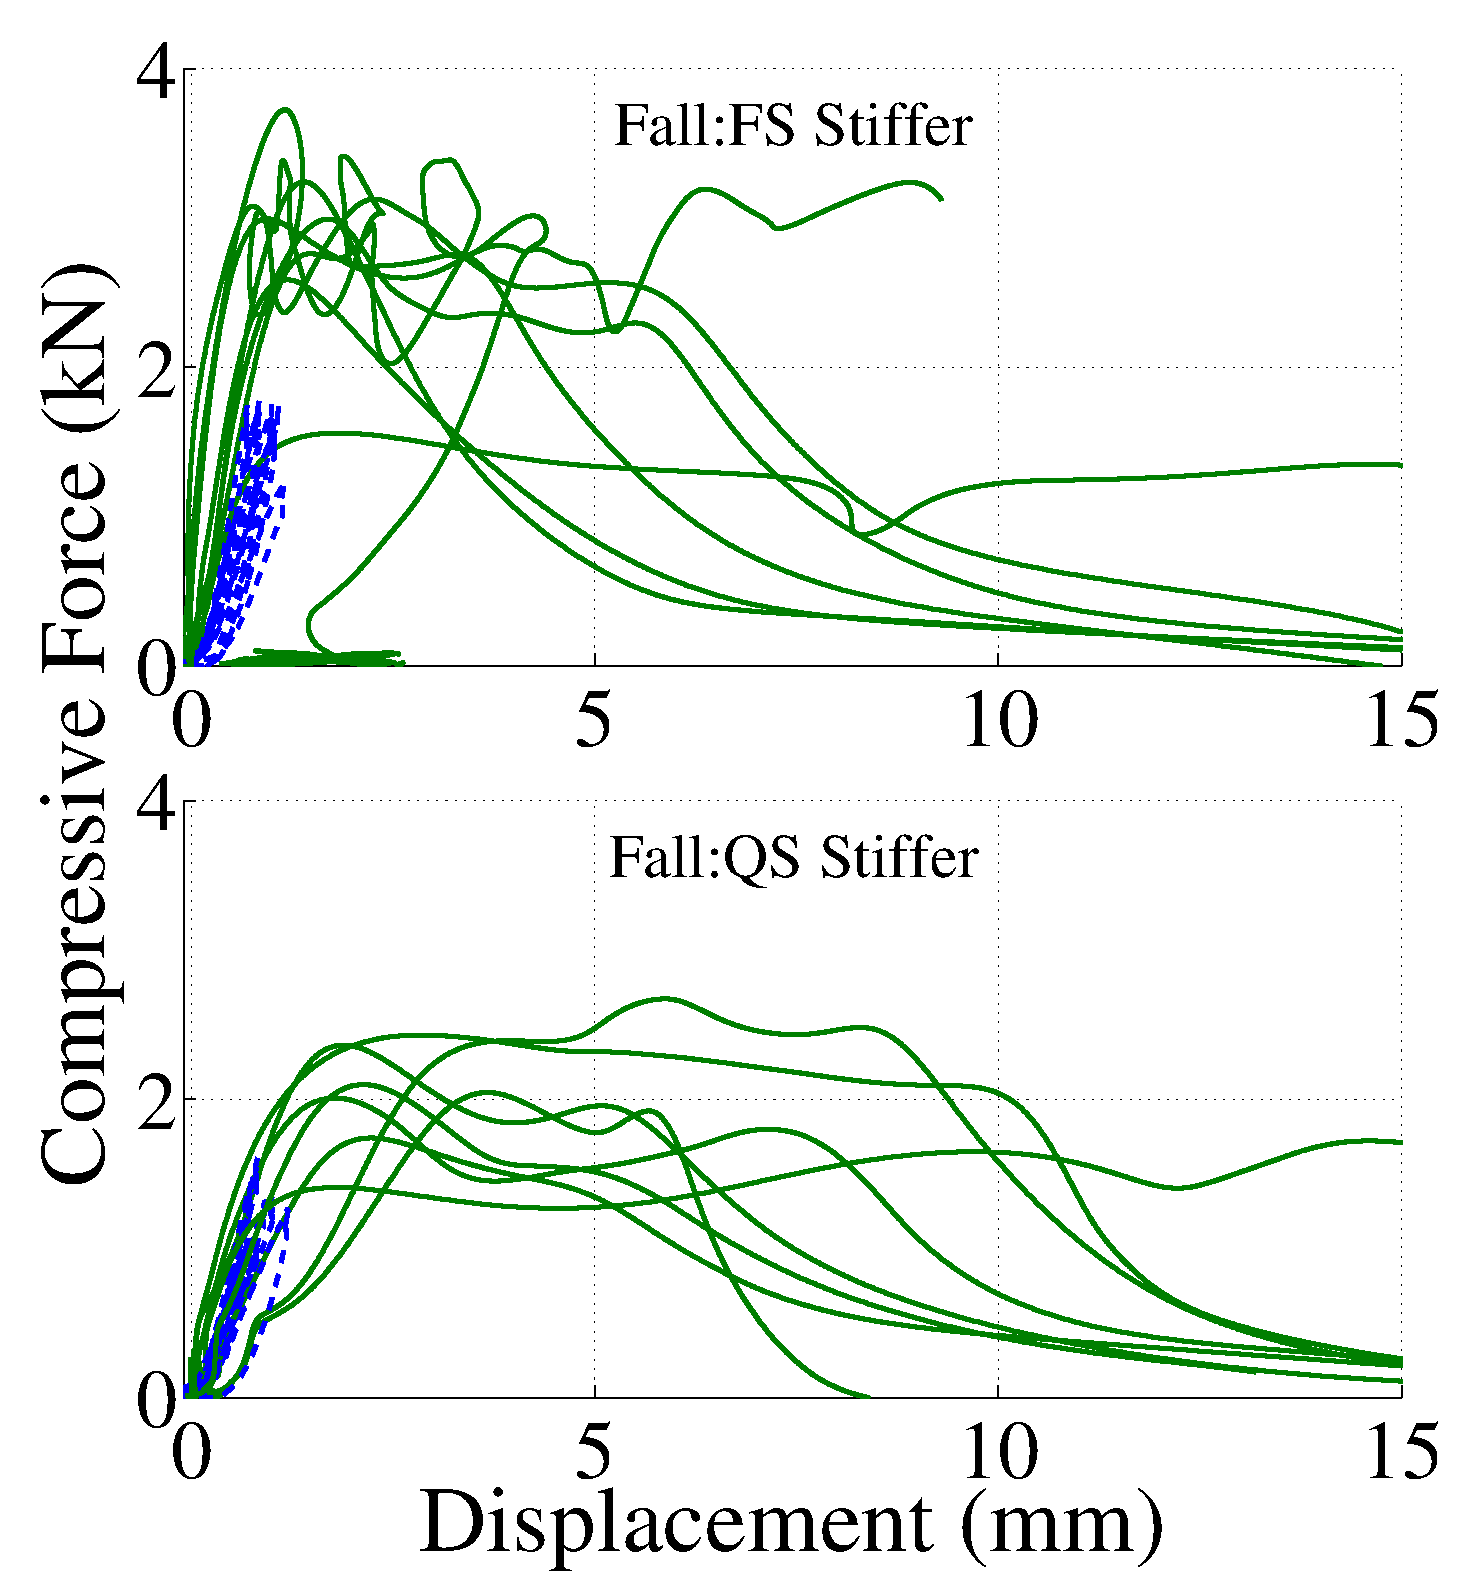
\includegraphics[width=\linewidth]{./behave_fail/Figures/Force_Disp_GroupedStiff}
\caption[Force-displacement behaviours grouped by relative stiffness of fall:\acs*{fs} and fall:\acs*{QS}]{
\textbf{Force-displacement curves for specimens, grouped by relative behaviour in the \ac{fs} and \ac{QS} conditions. Those that were stiffer in the \ac{QS} condition failed at a lower force, but displayed extended post yield behaviours. Dashed blue lines show the \ac{QS} loading response, and solid green lines are the \ac{fs} response.} Graphic \copyright Seth Gilchrist, 2013.}
\label{fig:Force_Disp_GroupedStiff}
\end{figure}

Yield force, stiffness and energy to fracture in the fall:\ac{fs} group were all significantly different from fast group (Table~\ref{tab:failData}).
The fall:\ac{fs} group was 24\% weaker, 160\% stiffer, and absorbed only 27\% of the energy before yielding.

\begin{table}
\centering
\begin{threeparttable}
\caption[Data for failure groups]{Data from the fall:\ac{fs}, fast and slow failure groups given as median (minimum, maximum) for non-normal data, and mean (standard deviation) for normally distributed data.}
\label{tab:failData}
\begin{tabular}{lccc}
\toprule
Measure 					& Fall:\ac{fs} 			& Fast				& Slow 					\\ \midrule
Yield Force (\ac{n})			 	& 2.39 (1.41, 3.72)	& 3.15 (2.17, 5.30)\tnote{*}	& 2.42 (1.46, 4.44)		\\ 
Stiffness (\ac{kn}/\ac{mm}) 			& 1.92 (1.20) 		& 0.74 (0.25)\tnote{*} 		& 1.66 (0.52)	 		\\ 
Energy (\acs{j}) 					& 2.55 (0.545, 5.39)& 9.33 (5.46, 15.4)\tnote{*}	& 4.38 (1.14, 12.2)\tnote{*}		\\
\bottomrule
\end{tabular}
\begin{tablenotes}
\item[*]{\footnotesize $p \leq 0.01$ compared to fall:\ac{fs}}
\end{tablenotes}
\end{threeparttable}
\end{table}

Energy in the fall:\ac{fs} group was significantly different from the slow group, absorbing only 58\% of the slow group's average before yield, but no differences were observed in yield force (\ac{pw}$ = 0.85$) or stiffness (\ac{pt}$ = 0.82$).

\begin{figure}
\centering
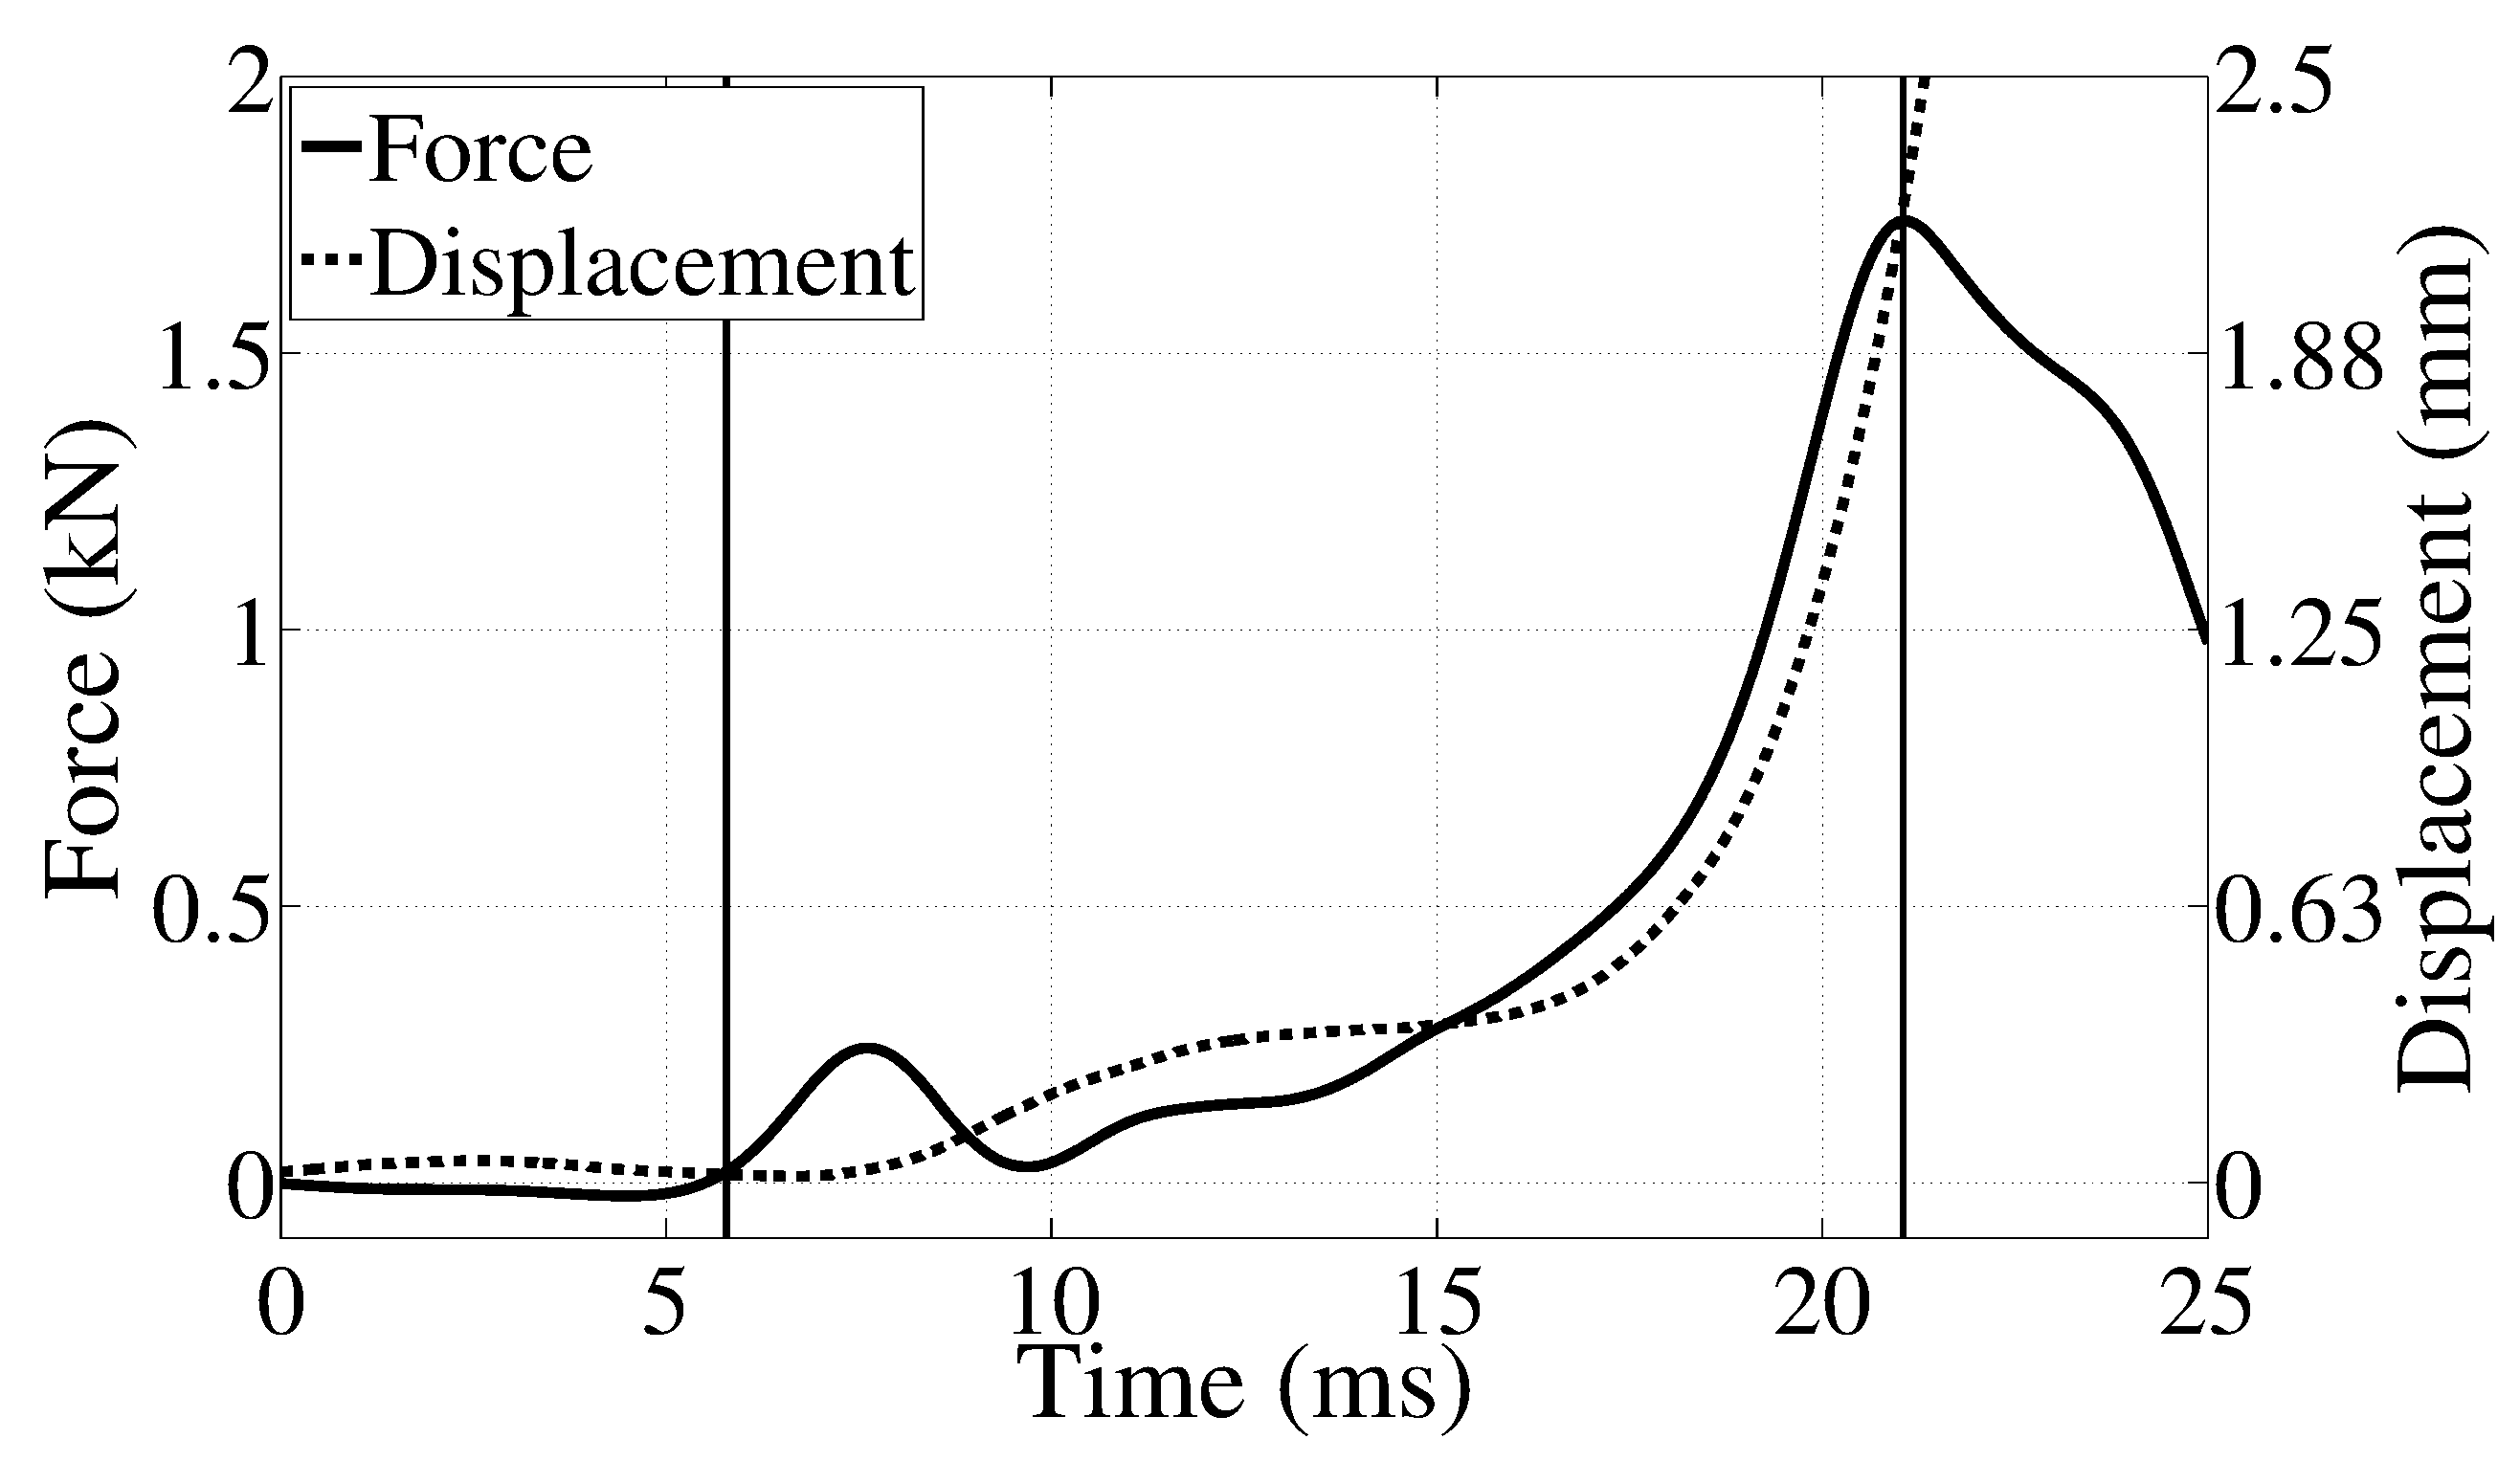
\includegraphics[width=\linewidth]{./behave_fail/Figures/Force_Disp_TimeExp}
\caption[Force and displacement \acs*{vs} time example]{\textbf{An example force and displacement \ac{vs} time plot. The vertical lines indicate the beginning of the impact (force $>$ 20~\ac{n}) and yield. Loading rate was defined as the average slope of the force-time curve from when the force exceeded 20~\ac{n} to yield. Likewise, displacement rate was the average slope of the displacement-time curve from when the force exceeded 20~\ac{n} to yield. These data are for specimen 7 and display the non-constant loading and displacement rates.} Graphic \copyright Seth Gilchrist, 2013.}
\label{fig:Force_Disp_TimeExp}
\end{figure}

The fall:\ac{fs} group displayed a variety of loading and displacement rates, both of which correlated with specimen stiffness (Table~\ref{tab:summary} and Figs.~\ref{fig:Force_Disp_TimeExp},~\ref{fig:StiffVsRate_HighRes} and~\ref{fig:Force_DispExp}).
As stiffness increased, loading rate increased (\ac{pt}$ < 0.01$) and displacement rate decreased (\ac{pt}$ < 0.01$).
Additionally, stiffness and yield force were proportionally related (\ac{pt}$ < 0.01$, \ac{r2}$ = 0.391$).
Finally, loading rate was correlated to maximum force (\ac{r2}$ =0.92$, \ac{pt}$ < 0.001$), but no correlation with displacement rate was observed (\ac{pt}$ = 0.16$).

\begin{figure}
\centering
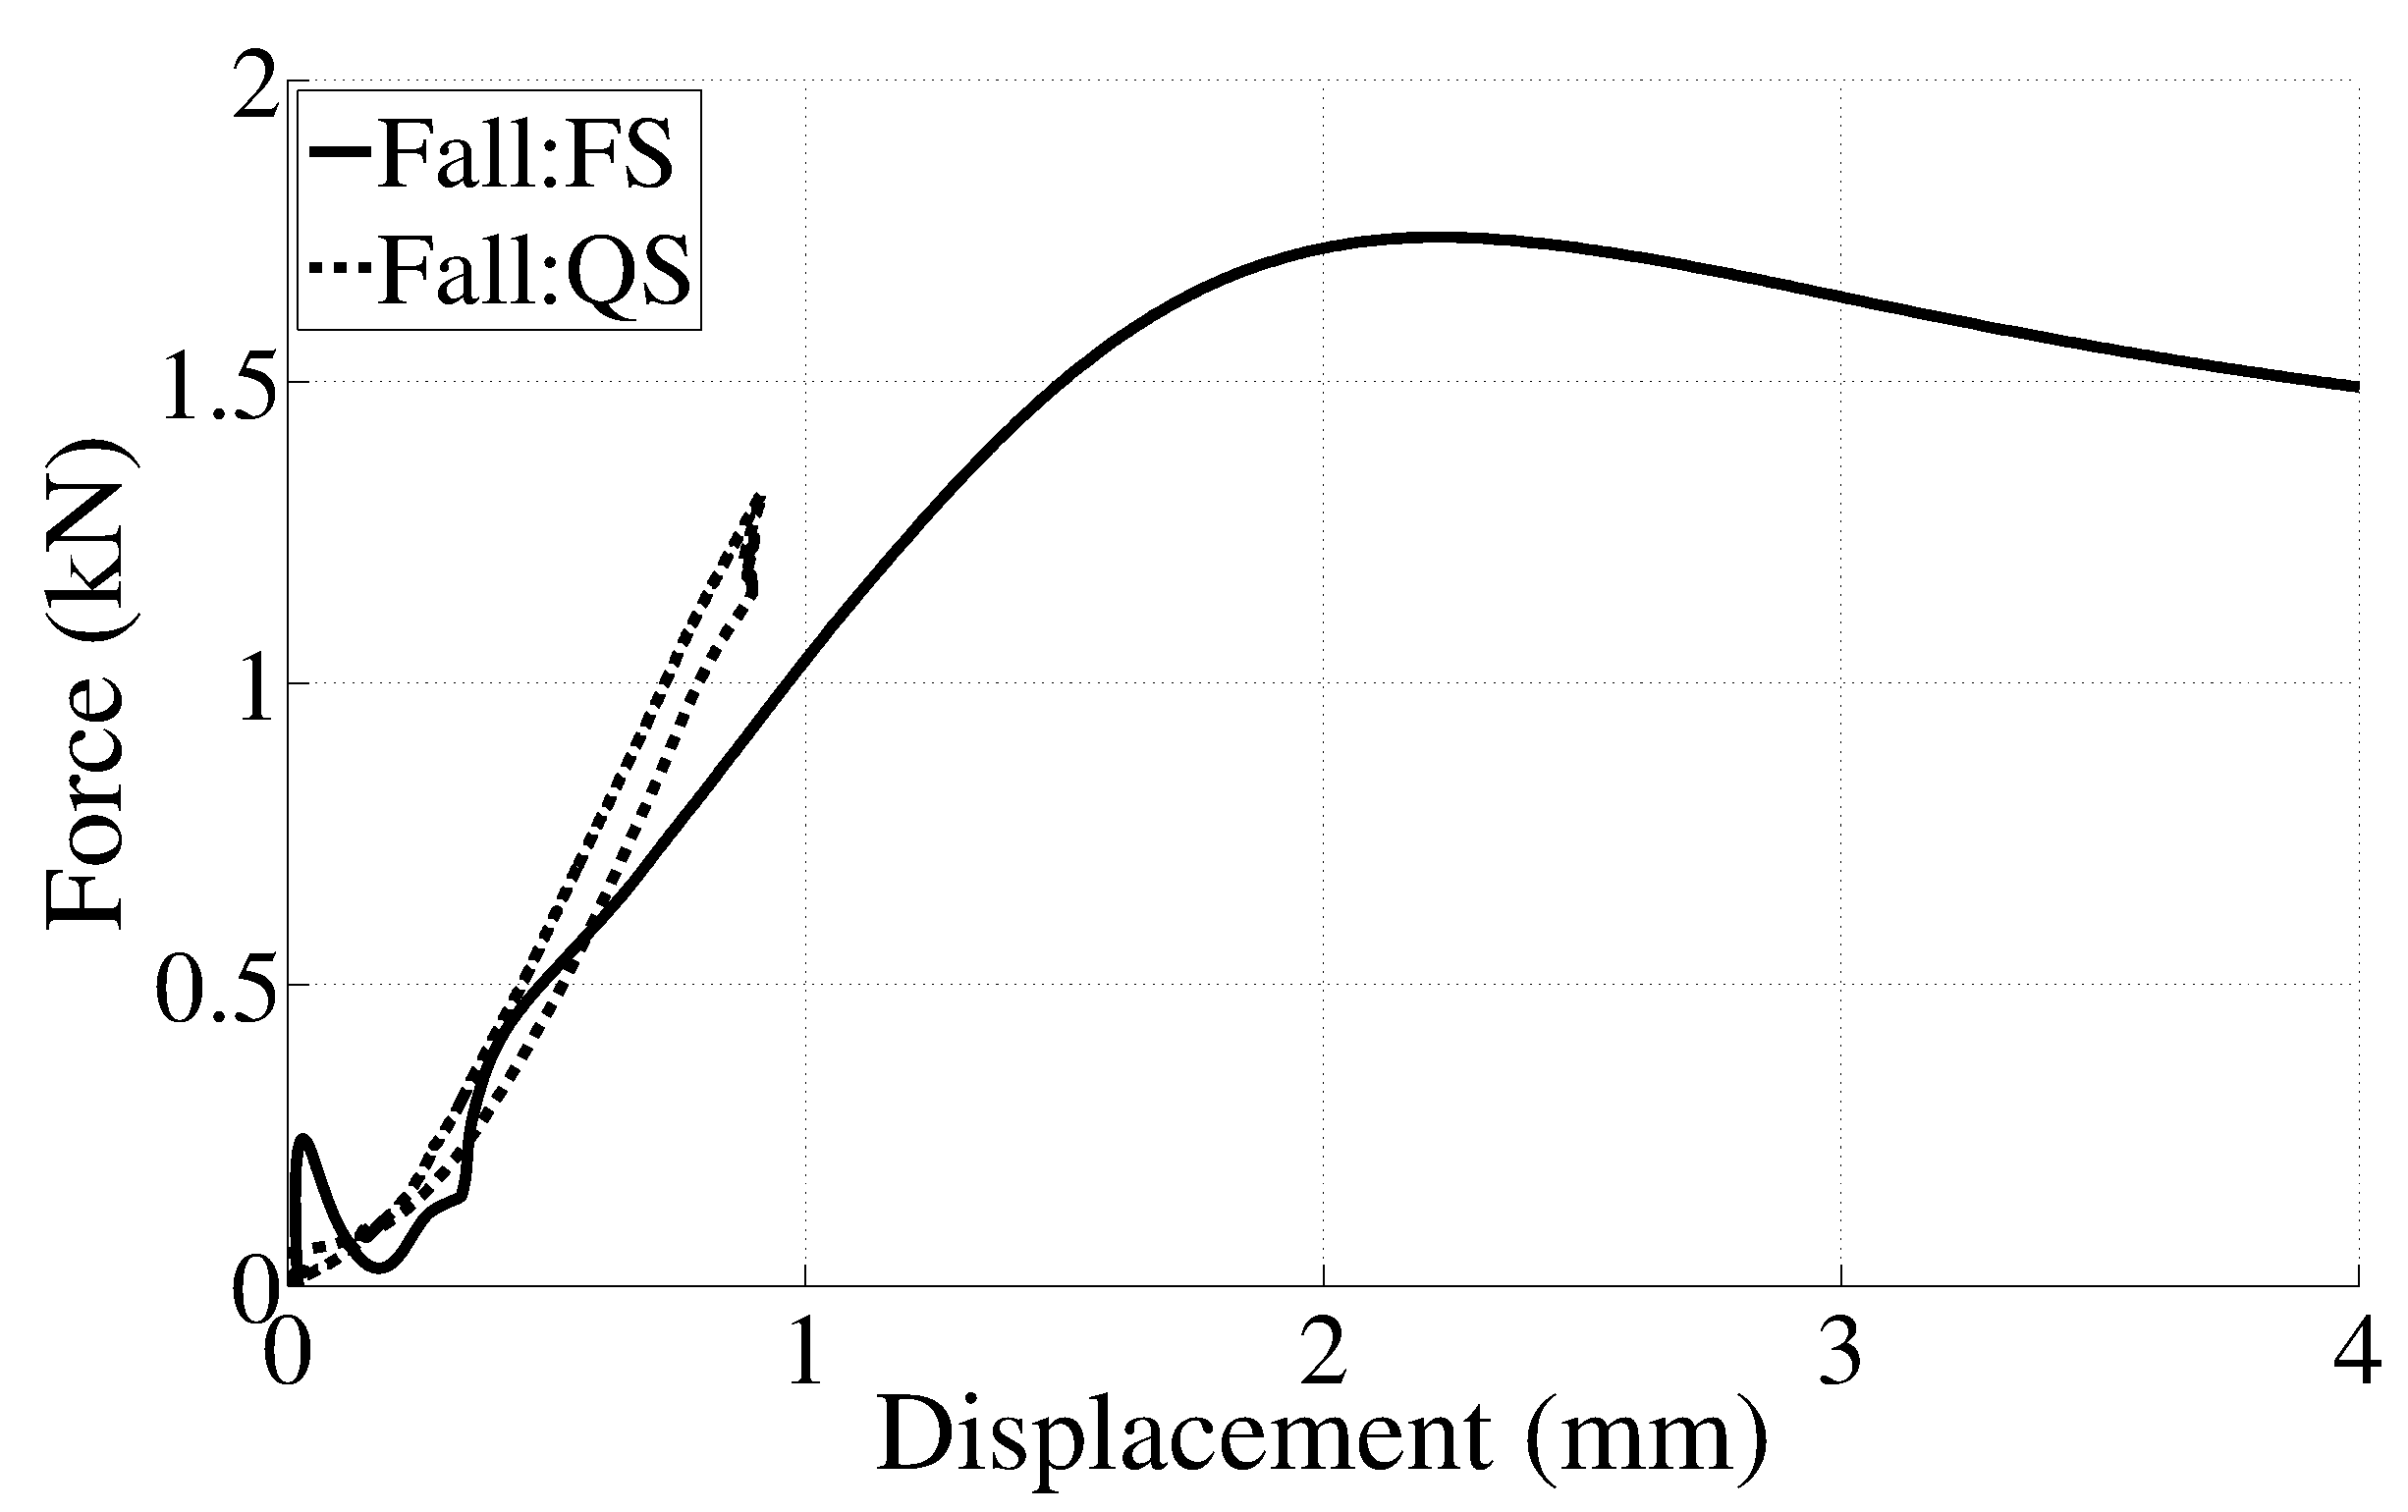
\includegraphics[width=\linewidth]{./behave_fail/Figures/Force_DispExp}
\caption[Force \acs*{vs} displacement example]{\textbf{An example force \ac{vs} displacement plot. In this case the quasi-static test had a higher stiffness than the fall simulation. These data are for specimen 7.} Graphic \copyright Seth Gilchrist, 2013.}
\label{fig:Force_DispExp}
\end{figure}

\begin{figure}
\centering
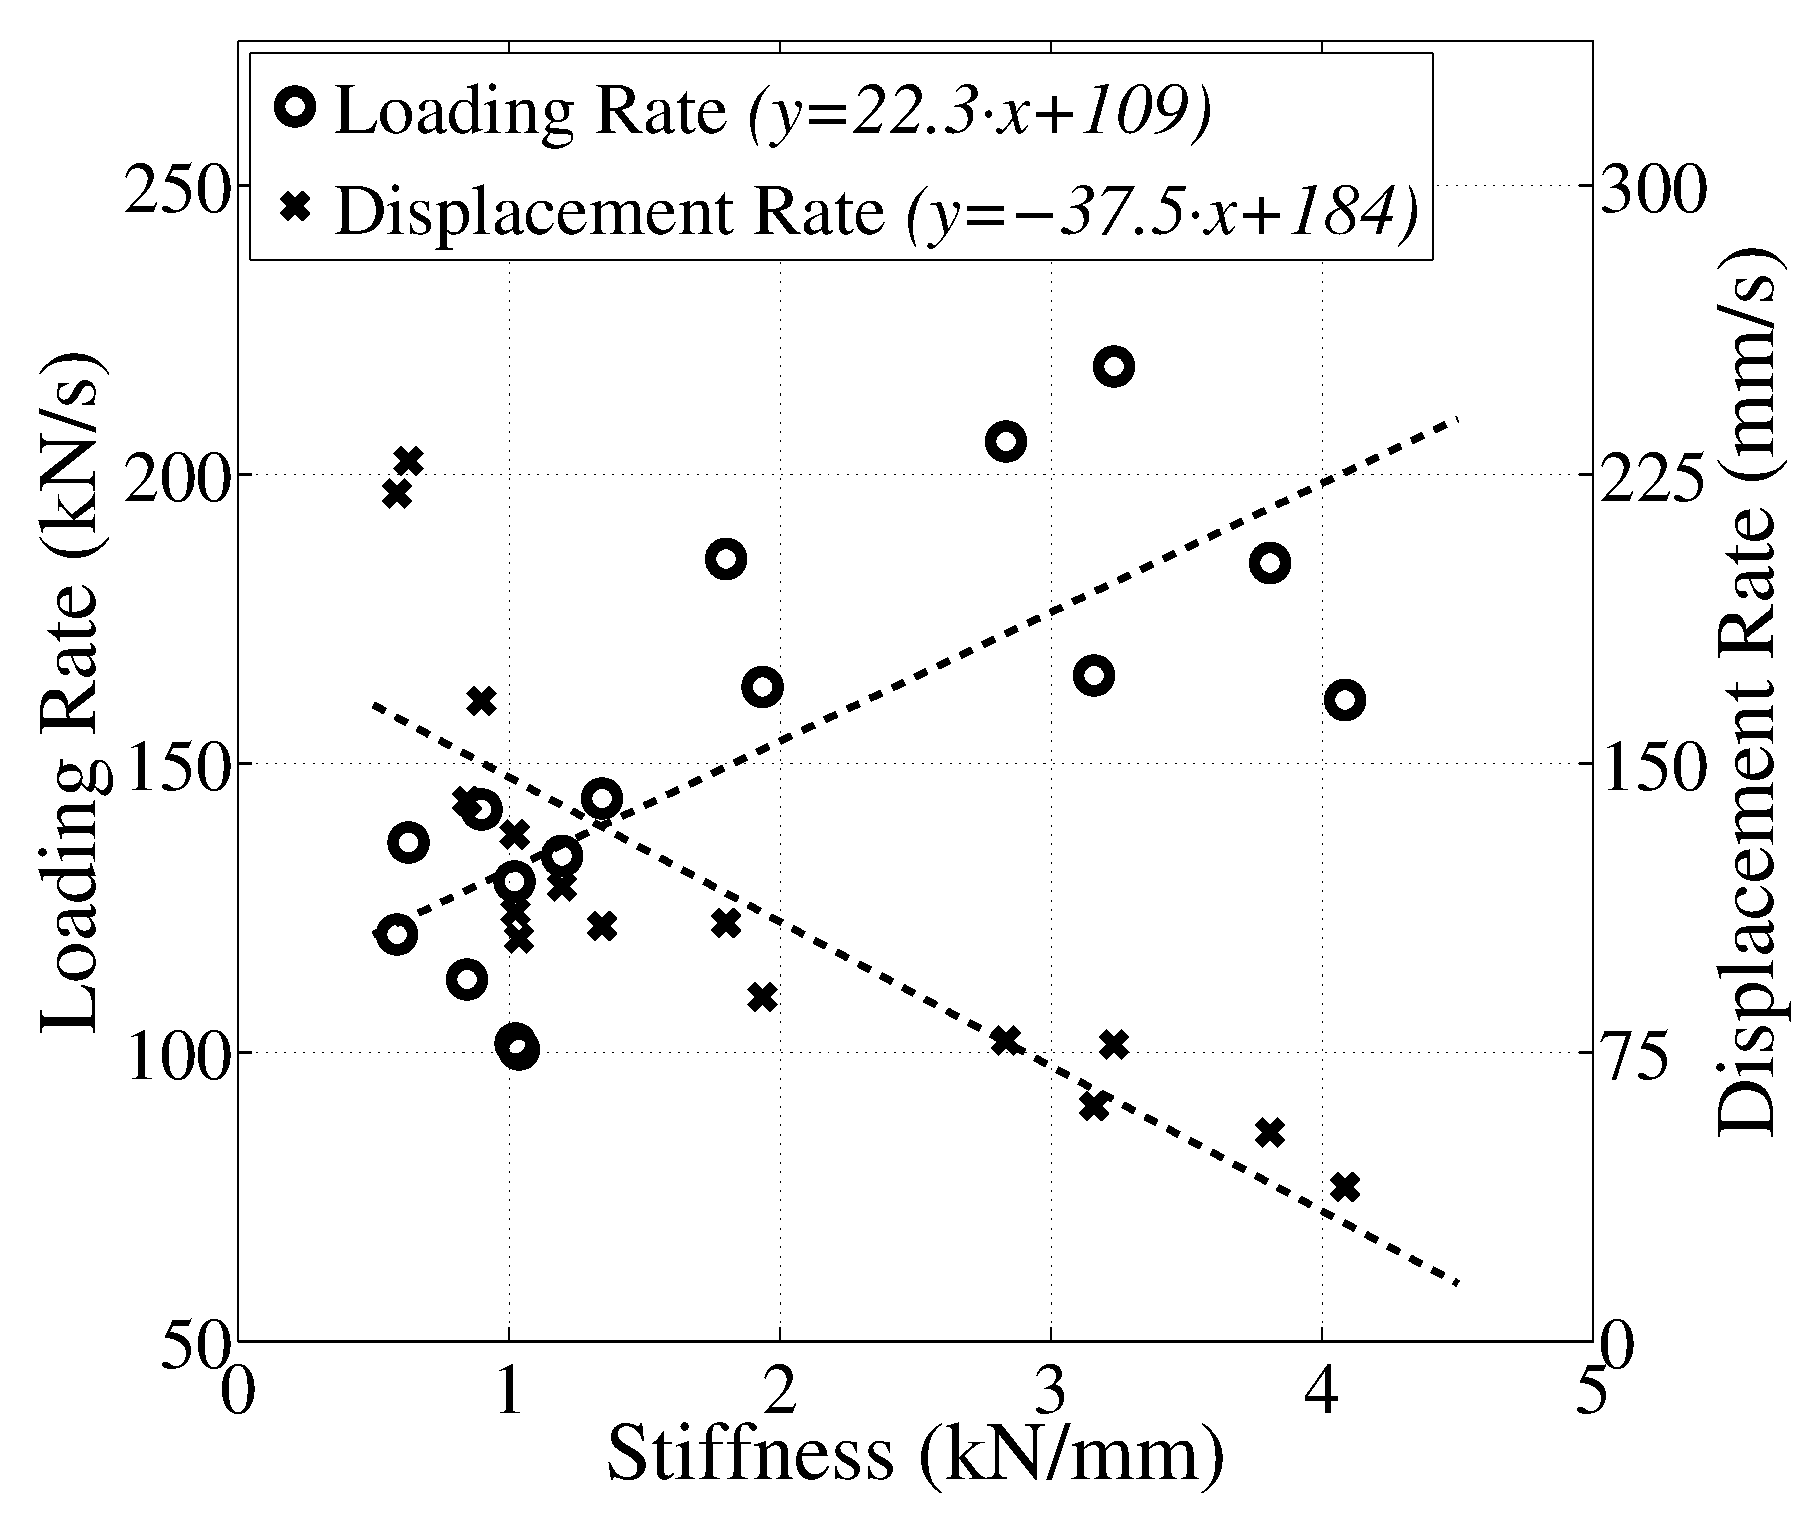
\includegraphics[width=\linewidth]{./behave_fail/Figures/StiffVsRate_HighRes}
\caption[Stiffness \acs*{vs} loading and displacement rates]{\textbf{Fall:\ac{fs} loading and displacement rates as functions of stiffness. Data points and regression lines for loading rate (\ac{r2}$ = .53$), and displacement rate (\ac{r2}$ = 0.66$) are shown.} Graphic \copyright Seth Gilchrist, 2013.}
\label{fig:StiffVsRate_HighRes}
\end{figure}

There were no differences in the slopes of the yield force \ac{vs} total \ac{abmd} regression lines between the fast, slow and fall:\ac{fs} groups (\ac{pt}$ = 0.88$ and \ac{pt}$ = 0.46$ for \citet{de_bakker_during_2009} and \citet{nishiyama_proximal_2013}, respectively). 

\section{Discussion}
\label{sec:behave_fail_discssion}
The goals of our experiments were three fold: i) to determine if there were differences in behaviour between quasi-static, constant displacement rate and fall simulation loading conditions; ii) to determine if there were differences in failure characteristics between constant displacement rate loading and fall simulation; and iii) to characterize the variation in loading and displacement rates as a function of specimen stiffness in the fall simulation tests.
Our fall:\ac{QS} \ac{vs} fall:\ac{fs} results dictate that we accept the null hypothesis that the sub-failure mechanical behaviour is the same between these test conditions.
However, the results of the constant displacement rate failure \ac{vs} fall simulation failure loading showed significant differences, requiring us to reject the null hypothesis of no difference between quasi-static and impact fall simulation failure characteristics.
In the fall simulation tests we found that the average displacement rate decreased with specimen stiffness, while the average loading rate increased.

\subsection{Fall group viscoelasticity}
\label{sec:behave_fail_discssion_relating}
The lack of differences in the fall:\ac{QS} \ac{vs} fall:\ac{fs} strain, energy and stiffness data is in contrast to previous work in hip fracture~\citep{weber_proximal_1992, courtney_effects_1994}, and could be seen to run counter to studies that have shown that bone, as a material, is viscoelastic~\citep{fois_study_2001, carter_compressive_1977}.
However, studies examining bone have shown that the viscoelastic effects are limited, and if bone viscoelasticity alone were responsible for the increase in stiffness seen by \citet{courtney_effects_1994}, the change in stiffness from 2 to 100~\ac{mm}/\ac{s} would be on the order of 25\%, rather than the 100\% observed.
The result in this study of increased \ac{abmd} being predictive of changes in stiffness could indicate that bone marrow space, which is presumably less in specimens with more trabecular bone, might be responsible for the changes in stiffness.
The material level studies suggest that the viscoelastic response of bone is connected to the organic matrix present~\citep{fois_study_2001}, which is unknown for the current specimen groups, and to hydrodynamic effects of bone marrow at high strain rates~\citep{carter_compressive_1977}.
In the fall simulation tests, the displacement rates were lower at the beginning of the test than at the end (Figure~\ref{fig:Force_DispExp}), but were still two orders of magnitude higher than for the fall:\ac{QS} group.
Therefore, our results suggest that our specimens were not exhibiting strong viscoelastic behaviour under these displacement rates, and this is the reason for the similar stiffnesses, energies and strains measured.

To examine the role of viscoelasticity, an idealized model (Figure~\ref{fig:ImpactModel}) was used to evaluate anticipated behaviours.
If the impact dynamics of the drop tower gantry and top of the spring are ignored, the initial velocity, $v(0)$, of Mass 1 can be calculated to be 2.9~\ac{m}/\ac{s} using energy methods (\S\ref{sec:support_mass1_velocity}).
The soft tissue model significantly influences the shape of the force pulse, $f(t)$, delivered to Mass 2 and since the soft tissue is omitted in this model, a representative sinusoidal pulse of 250~\ac{n} over 5~\ac{ms} $ \left( f(t) = 250 \sin(\frac{2\pi}{0.01} \cdot t)\right) $ was used.
If the damping of the proximal femur is given a value of 0, and the pelvis spring is given its laboratory measured stiffness of 50~\ac{kn}/\ac{m}, the response of the system is similar to that seen in the actual tests (Figs.~\ref{fig:StiffVsRate_HighRes} and~\ref{fig:stiffVsRatesIdeal}). Computer code for this model can be found in \S\ref{sec:code_ideal_fs}.

\begin{figure}
\centering
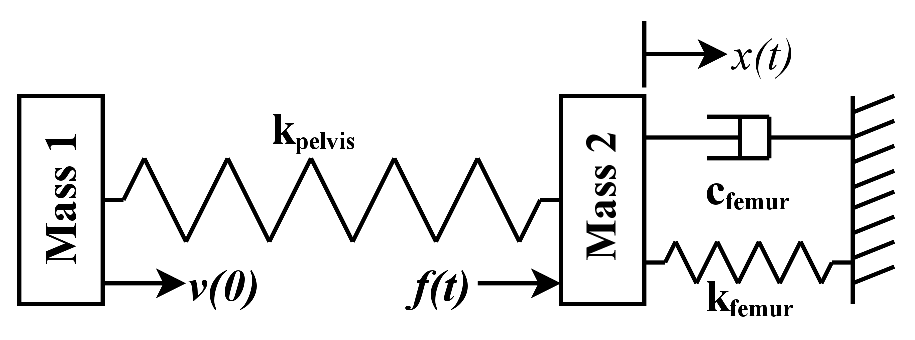
\includegraphics[width=\linewidth]{./behave_fail/Figures/ImpactModel}
\caption[Idealized model of the fall simulator]{\textbf{The impact fall simulator can be idealized using a series of two springs. This model is a 2~degree of freedom, second order model. It omits the soft tissue and models the pelvis spring as an ideal spring, and the femur as a spring and damper in parallel. Mass 1 is the combination of the body mass and the top third of the spring mass, and Mass 2 is the combination of the apparatus, bottom third of the spring, and the pelvis mass.} Graphic \copyright Seth Gilchrist, 2013.}
\label{fig:ImpactModel}
\end{figure}

\begin{figure}
\centering
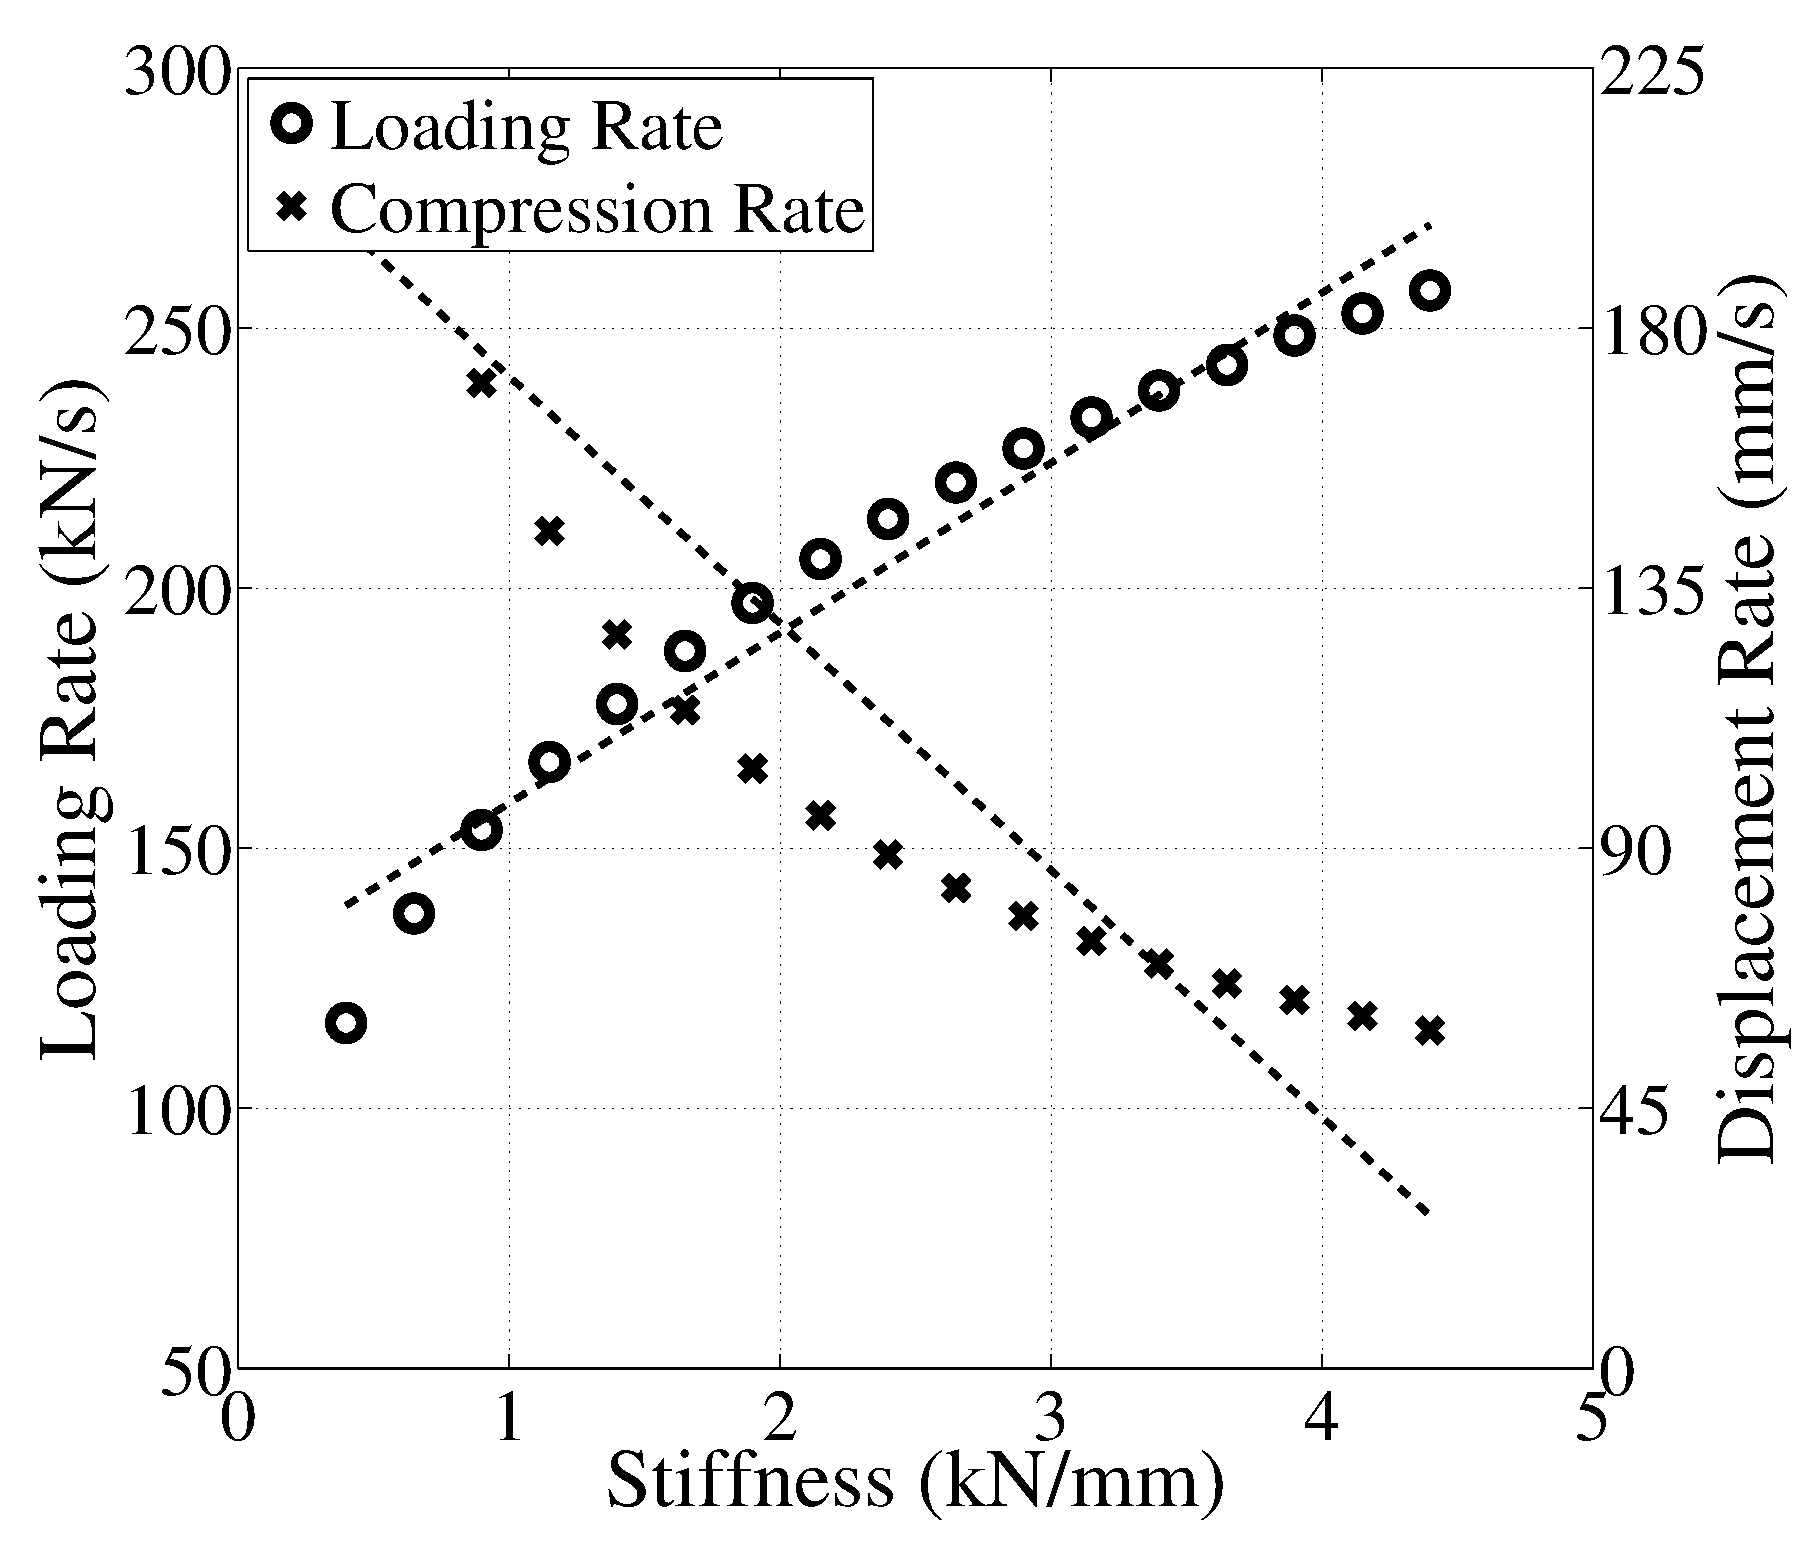
\includegraphics[width=0.7\linewidth]{./behave_fail/Figures/stiffVsRatesIdeal}
\caption[Ideal loading and compression rates \acs*{vs} stiffness]{\textbf{A plot for comparison to Figure~\ref{fig:StiffVsRate_HighRes} that shows the loading and compression rates \ac{vs} stiffness for an ideal spring-mass system up to 1500~\ac{n} of compressive force. The trend lines in this plot behave in the same manner to those in the experimental data, indicating that the system is behaving in a spring-like fashion.} Graphic \copyright Seth Gilchrist, 2013.}
\label{fig:stiffVsRatesIdeal}
\end{figure}

The question then becomes, what would the system look like if damping was increased, simulating high bone viscoelasticity?
The same model as above was used, however the force on Mass 2 was omitted because oscillations due to the force pulse were seen to dominate loading and displacement \ac{vs} stiffness plots at high damping levels.
Since none of the specimens were fractured by the initial force pules, the artefact created by it would obfuscate the important signals in the plots.
Therefore, the initial conditions were set to $v(0) = 2.9$~\ac{m}/\ac{s} and $f(0) = 0 $, and a number of different damping values were tested (Figure~\ref{fig:ratesVsDamping}).

\begin{figure}
\centering
\includegraphics[width=\linewidth]{./behave_fail/Figures/ratesVsDamping}
\caption[Ideal loading and displacement rates as a function stiffness and damping]{\textbf{Loading and displacement rates \acs{vs} stiffness, plotted for four different damping levels. The number in the upper left of each plot gives the value of $c_{femur}$.} Graphic \copyright Seth Gilchrist, 2013.}
\label{fig:ratesVsDamping}
\end{figure}

Increased damping has a large effect on the shape of the displacement rate curve, tending to flatten it out and decrease its overall value.
This shape change is due to the viscous element preventing compression of the spring element.
In specimens with low stiffness velocity tends to increase rapidly in the absence of damping, leading to high displacement rates.
However, in situations where the viscous response dominates, high compressions are never achieved.
Increasing the damping decrease the value of the loading rate curve and, at higher damping levels, flattens out the response.
This flattening of the load and displacement rate curves at high damping levels occurs because the system is over damped.
In the over damped scenario, the loading rate tends towards a constant value, determined by the compression rate of the pelvis spring, and the displacement rate tends to a value of zero.

In the test results (Figure~\ref{fig:StiffVsRate_HighRes}) the loading rate fit line has a positive slope, and the displacement rate fit line has a negative slope, leading us to draw the conclusion that viscoelastic response is likely minimal.

So how does this fit in with the work of \citet{courtney_effects_1994}?
The change in stiffness reported by \citet{courtney_effects_1994} for old femurs was an increase of 92\% when increasing the displacement rate from 2~to 100~\ac{mm}/\ac{s}.
These data can be used to estimate the damping coefficient of their specimens.
Modelling the system used by \citet{courtney_effects_1994} as a spring and damper in parallel, driven by a constant displacement rate (Figure~\ref{fig:courtneyModel}), we can estimate the damping coefficient needed to double the stiffness to a given compressive force (equations for this analysis cab be found in \S\ref{sec:support_courtney_response}).

\begin{figure}
\centering
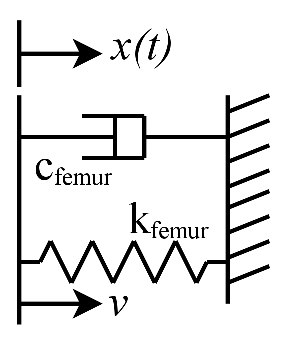
\includegraphics[width=0.3\linewidth]{./behave_fail/Figures/courtneyModel}
\caption[Idealized \citet{courtney_effects_1994} model]{\textbf{An idealized version of the test setup used by \citet{courtney_effects_1994}. The stiffness of the construct is the combination of the baseline femur stiffness and the resistance due to the damping.} Graphic \copyright Seth Gilchrist, 2013.}
\label{fig:courtneyModel}
\end{figure}

Using a baseline femoral stiffness of 1.5~\ac{kn}/\ac{mm} (which is similar to the 2~\ac{mm}/\ac{s} value measured by \citet{courtney_effects_1994}) and calculating the stiffness up to 2.4~\ac{kn} (the average strength of the current specimens) shows that to double the stiffness when displacement rate is changed from~2 to~100~\ac{mm}/\ac{s}, the damping coefficient, c$_{femur}$ would need to be approximately 12~\ac{n}\ac{s}/\ac{mm} (Figure~\ref{fig:courtneyDamping}).
If, however, the bone was acting in accordance to the strain rate to the power of 0.047-0.06~\citep{carter_compressive_1977, linde_mechanical_1991, crowninshield_response_1974}, the corresponding damping coefficient would be approximately 5~\ac{n}\ac{s}/\ac{mm}.

\begin{figure}
\centering
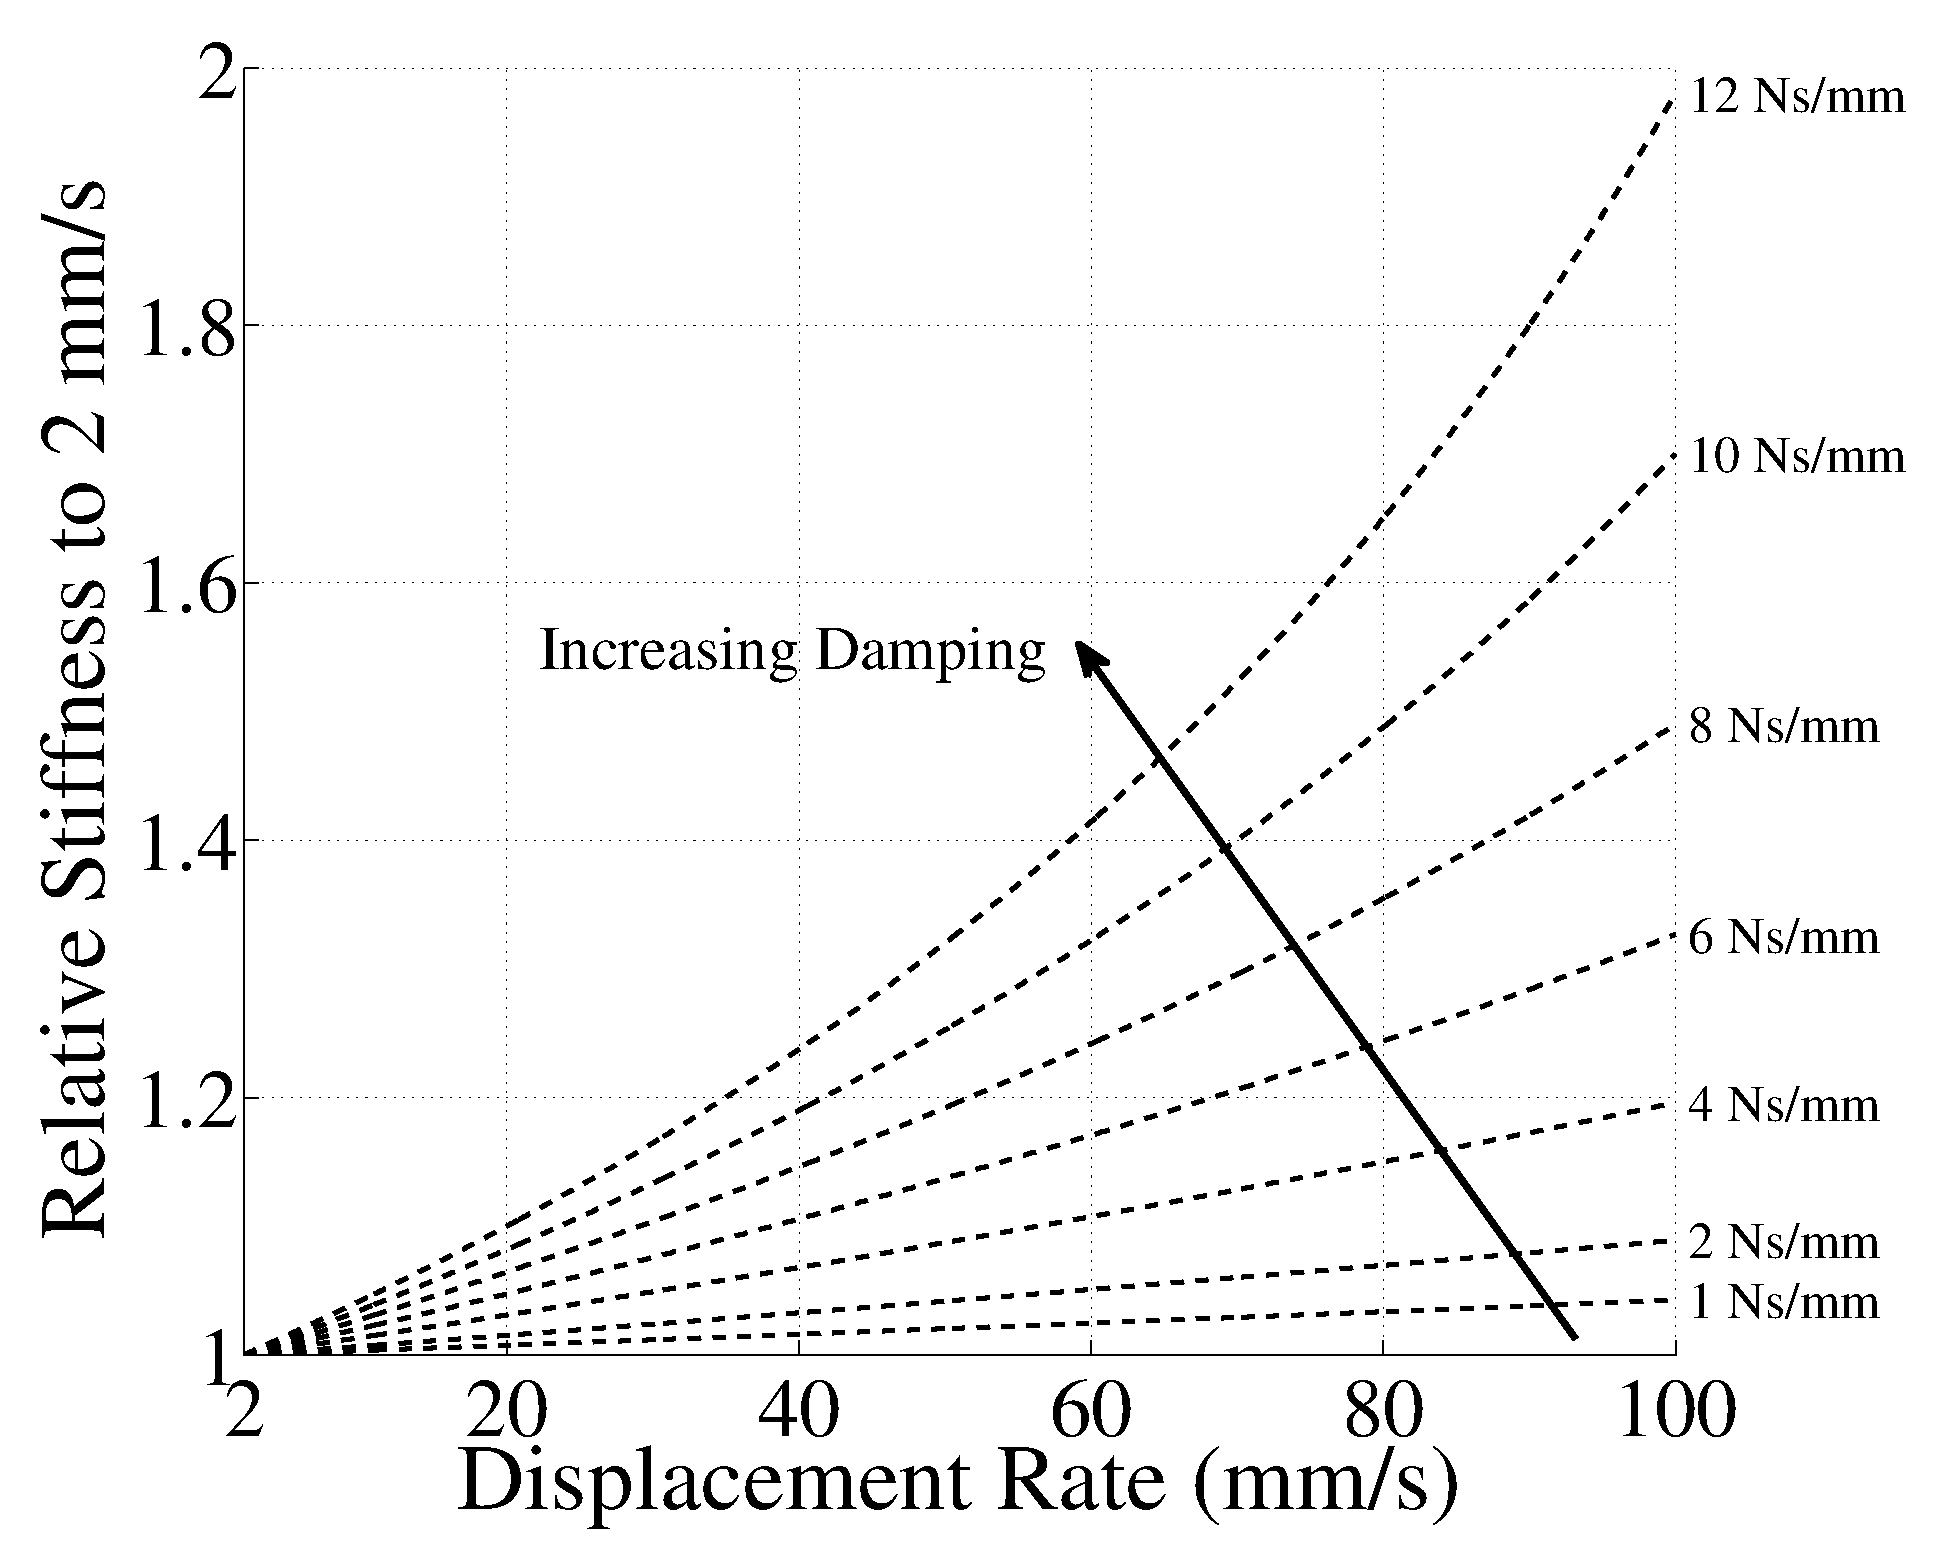
\includegraphics[width=0.7\linewidth]{./behave_fail/Figures/courtneyDamping}
\caption[Stiffness \acs*{vs} displacement rate and damping]{\textbf{Stiffness relative to the 2~\ac{mm}/\ac{s} value as displacement rate increases for various damping coefficients. Relative stiffness was calculated to a force of 2.5~\ac{kn}. Selection of target force or target displacement is important as it changes the nature of the relationship} (\S\ref{sec:support_courtney_response}). Graphic \copyright Seth Gilchrist, 2013.}
\label{fig:courtneyDamping}
\end{figure}

Returning now to the model of the current experiment, it can be seen that if the bone viscoelasticity was on the order of 5~\ac{n}\ac{s}/\ac{mm}, as proposed by \citet{carter_compressive_1977}, \citet{linde_mechanical_1991} and \citet{crowninshield_response_1974}, then it might be difficult to determine if the specimens in the current tests are acting with that level of viscoelasticity.
The model's displacement rate has a distinct negative slope, as does the experiment's, and there is considerable variation in the experiment's loading rate values, which might hide a lower slope than the fit line, similar to the model's.
However, if the specimens are acting with the level of viscoelasticity noted by \citet{courtney_effects_1994}, then one might anticipate nearly constant displacement and loading rates for all specimens, regardless of their baseline stiffnesses.
\citet{courtney_effects_1994} saw that young specimens with a higher baseline stiffness also doubled their stiffness at the higher displacement rates, indicating that their results were consistent regardless of baseline stiffness.
From this, we can conclude that the specimens may have some viscoelastic behaviour, but in the current tests it is not strong enough to heavily influence the response.

\subsection{Failure and loading responses in the fall simulator}
\label{sec:behave_fail_discssion_fail}
The fall:\ac{fs} group was significantly different from the fast group in every measure.
In absolute value terms the yield force was not much different, but the low stiffness in the fast group meant that the energy absorbed was higher.
The mechanism for these differences is not known, but the lower stiffness and higher yield force are incongruent with anticipated viscoelastic effects.

A central result of the study was observation of the variable nature of displacement and loading rates during a fall to the side.
Previous investigators have evaluated the effects of displacement rate by testing specimens to failure under multiple, fixed displacement rates~\citep{courtney_effects_1994, weber_proximal_1992}.
A consequence of fixing the displacement rate is that all specimens, even the stiff ones, are exposed to high loading rates.
The average stiffness from \citet{courtney_effects_1994} of 3.0~\ac{kn}/\ac{mm} at 100~\ac{mm}/\ac{s}, results in a loading rate of 300~\ac{kn}/\ac{s}.
Previous researchers have estimated the peak loading rate in humans falling to the side to be approximately 100~\ac{kn}/\ac{s}~\citep{laing_characterizing_2010}.
The current tests include a compliant pelvis model which acted to mitigate extreme loading rates, leading to an average rate of 150~\ac{kn}/\ac{s}.
Enforcing a high displacement rate on specimens may reduce the biofidelity when compared to free response.
While loading rates of 300 and 100~\ac{kn}/\ac{s} are the same order of magnitude, the differences could affect specimen behaviour in ways that are difficult to predict given the complex geometry and bone material response~\citep{carter_compressive_1977, robertson_compressive_1978, linde_mechanical_1991, hansen_effect_2008, zioupos_microcracking_2008}.

In the fall:\ac{fs} group, displacement rate was related to stiffness, but not to yield force.
While a statistical relationship with yield force could not be found, this could be due to a lack of power since the post hoc power of the current experiment is only 0.28.
The inverse relationship between stiffness and displacement rate contradicts the outcomes of previous research~\citep{courtney_effects_1994, weber_proximal_1992}.
This is thought to be a result of the influence of specimen stiffness on the dynamic response.
In the dynamic situation that we studied, displacement rate is related to specimen stiffness, with softer specimens experiencing higher displacement rates, which is in agreement with the fundamental mechanics of an undamped, spring-mass system.
We believe that observations of previous researchers~\citep{courtney_effects_1994, weber_proximal_1992}, who noted an increase in stiffness as displacement rate increased, were potentially an artefact of the prescribed constant loading rates on the bones.

\subsection{Conclusions}
\label{sec:behave_fail_discssion_conclusions}
Our approach here is markedly different from previous hip fracture fall simulation tests and we believe that it incorporates important improvements over the previous test methods in terms of concordance between the loading situation in real world falls and those in the experiment.
Most importantly, the new test method produces both loading and displacement rates as outcome variables that are determined by the biomechanics of the fall and bone structural material properties, rather than dictating one of these parameters a priori.
Secondly, the use of the same specimen to test two different loading conditions improves statistical power to assess the differences in mechanical behaviours.

While the advantages of the current method are important, there are also limitations with respect to comparison to previous studies.
The lack of match pairs for failure mechanics comparison reduced our ability to show differences in failure behaviours.
However, comparisons were made to two populations of specimens that were similar to the current one.
Additionally, specimens were from a non-fracture population, which may reduce the ability to identify mechanics of bones that actually fracture due to a fall.
Further, only surface strain and force-displacement behaviours were assessed, with no insight into the internal mechanics and load sharing between cancellous and cortical bone.
This final point is best addressed through the use of computational modelling, which is currently on-going.
Notably, the finite element models are developed and validated using data from the fall:\ac{QS} group.
Once the models have been validated for sub-failure loading using that data (for which no differences were seen vis-a-vis the fall:\ac{fs} group), they will be extended to model the failures observed in the fall:\ac{fs} group.

This chapter has shown that the mechanical behaviour of the proximal femur is the same in quasi-static, constant displacement rate loading as it is in impact fall simulation.
However, it has also shown that prescription of a single displacement rate at the greater trochanter for all specimens is a simplification that could significantly alter the behaviour of the specimen and may have been responsible for the viscoelasticity observed by previous researchers.
The following chapter will address the strain and failure characteristics of the proximal femur in the two loading scenarios, addressing the last two research questions outlined in Section~\ref{sec:intro_goals_questions}.